\subsection{Arquitecturas de Red}

Los componentes de los sistemas de detección de intrusos pueden ser conectados entre sí, a través de las redes que los implementa o a través de redes separadas estrictamente diseñadas para la comunicación entre estos componentes, así evitando una conexión desde redes no autorizadas a los componentes. A la red dedicada para la comunicación de estos componentes es conocida como \textit{Red de administración} (ver Figura \ref{fig:red_admon}), en donde los sensores o agentes son administrados a través de la red de administración (zona dentro del recuadro rojo). En caso de que la organización no pueda crear una red aislada para dicha comunicación, cada sensor o agente del host debe tener una red virtual aislada para su comunicación. A esta red virtual implementada, en lugar de la red física aislada, se le conoce como \textit{interfaz de administración} (ver Figura \ref{fig:interfaz_admon}). Así, los agentes o sensores no pueden pasar información entre redes ni interfaces, haciendo que los servidores de administración, bases de datos y consolas estén únicamente apegadas a la red de administración. Los beneficios de realizar dicha separación de redes, es ocultar la existencia de un IDS dentro de la red de la organización a una contra parte, la protección del IDS ante ataques y asegurar una banda de ancho adecuada para su funcionamiento. Las desventajas que se generan al emplear esta arquitectura, son: incremento del costo para la creación de las redes y la inconveniencia para los usuarios y administradores del sistema para la administración del mismo, pues dicha administración se encuentra en diferentes equipos de cómputo.
	
	
\begin{figure}
\centering
\begin{subfigure}{.5\textwidth}
  \centering
  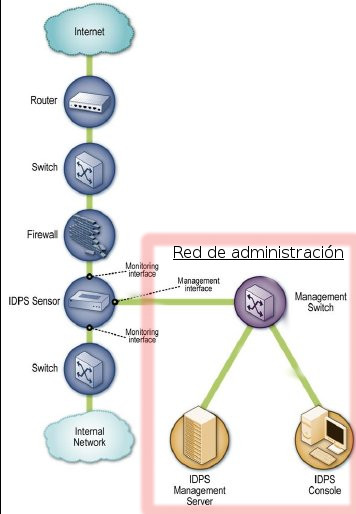
\includegraphics[scale=.7]{images/red_admon}
  \caption{Arquitectura de una red de administración.}
  \label{fig:red_admon}
\end{subfigure}%
\begin{subfigure}{.5\textwidth}
  \centering
  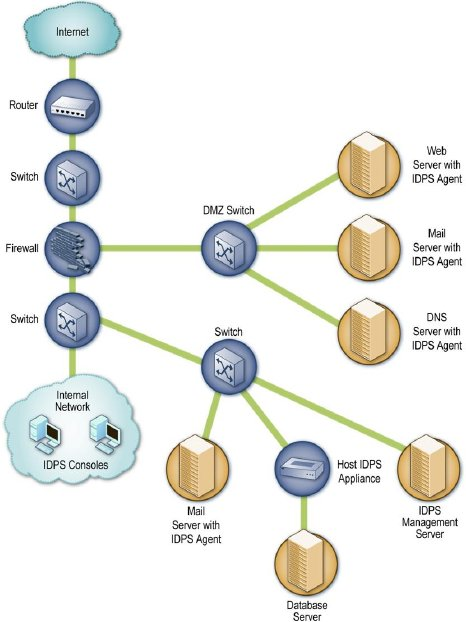
\includegraphics[scale=.55]{images/interfaz_admon}
  \caption{Arquitectura de una interfaz de administración implementada en la red de producción.}
  \label{fig:interfaz_admon}
\end{subfigure}
\caption{Arquitecturas de Red}
\label{fig:Arq_red}
\end{figure}
